\begin{rem}
We describe here some modifications we applied to the algorithm given in \cite{Danz02}.
\begin{enumerate}
\item In \cite{Danz02}, the corresponding constant \( U_{13,2} \) satisfies
\[
U_{13,2} = \max \{ |u_{r,2}'| \mid r \in \mathbb{N} \}.
\]
As shown in the proof, we relaxed this condition by replacing it with the inequality
\[
U_{13,2} \geq \max \{ |u_{r,2}'| \mid r \in \mathbb{N} \}.
\]
This relaxation still achieves the desired result. The main advantage of using the exact value is that it may satisfy Danzer’s criterion~\ref{eq:danzer} for a smaller \( r \). This is evident in Table~\ref{tab:proofn=13}, where the increasing behavior of \( |w_{r,2}'| \) begins from \( r = 1 \). However, determining \( \max \{ |u_{r,2}'| \mid r \in \mathbb{N} \} \) requires iterating the substitution on the edge \( \overline{OB_{1}} \) until all exact values of \( t_r \) are obtained, which is more labor-intensive than simply considering the maximum \textit{possible} value of \( |u_{r,2}'| \).

\item The matrix \(M_1\) in \cite{Danz02}, which was used to obtain the minimal polynomial (and is equivalent to \(M_n\) in this work), is the substitution matrix of the one-dimensional substitution on the set of edges naturally induced by the substitution rule. For convenience, we did not use such a matrix here, since \(M_n\) already contains all the relevant information for the proof, such as the minimal polynomial and the eigenvector containing the lengths of all prototile edges.

\item We did not explicitly use condition (A3) (in our notation, this is $\dfrac{|\overline{A_1B_1}|}{|\overline{OB_1}|} \notin \mathbb{Q}(\mu_n)$) in \cite{Danz02}. This is because each edge length \(s_{n,j}\) (see Lemma~\ref{lem:s_n,j}) and \(|OB_{n,1}|\) lies in \(\mathbb{Z}[\mu_n]\), which in turn implies, by the closure property, that \(|OB_{n,r}| \in \mathbb{Z}[\mu_n]\) for all \(r\). This is precisely the reason why (A3) is included as a condition in \cite{Danz02}, and hence it is not necessary in our proof.
\end{enumerate}
\end{rem}

\begin{conj}
\label{thm:Conjecture1}
During the calculation of the characteristic polynomial $p_n (x)$, a pattern in its coefficients becomes apparent. This polynomial can be expressed as $p_n (x)=-(x-1) q_n (x)$, where the coefficients of $q_n (x)$ in standard form follow the pattern described in Figure~\ref{fig:pattern}, at least for the given values of $n$. The signs of the coefficients from left to right follow a specific sequence: $+,-,-,+,+,-,-,+,+,\ldots$ The last two coefficients in each row are equal to either $1$ or $-1$, depending on $n$. The remaining coefficients are obtained by summing the absolute values of the two numbers indicated by the adjacent segments of the same color, then assigning the appropriate signs according to their positions. Clearly, the minimal polynomial $g_n (x)$ is equal to $q_n (x)$ if $q_n (x)$ is irreducible. An analogous pattern exists for the cases $n\in \{7,11,15,19,23,27,31\}$, and it is the author’s conjecture that this pattern holds for all odd $n\geq 5.$
\end{conj}

\begin{figure}[H]
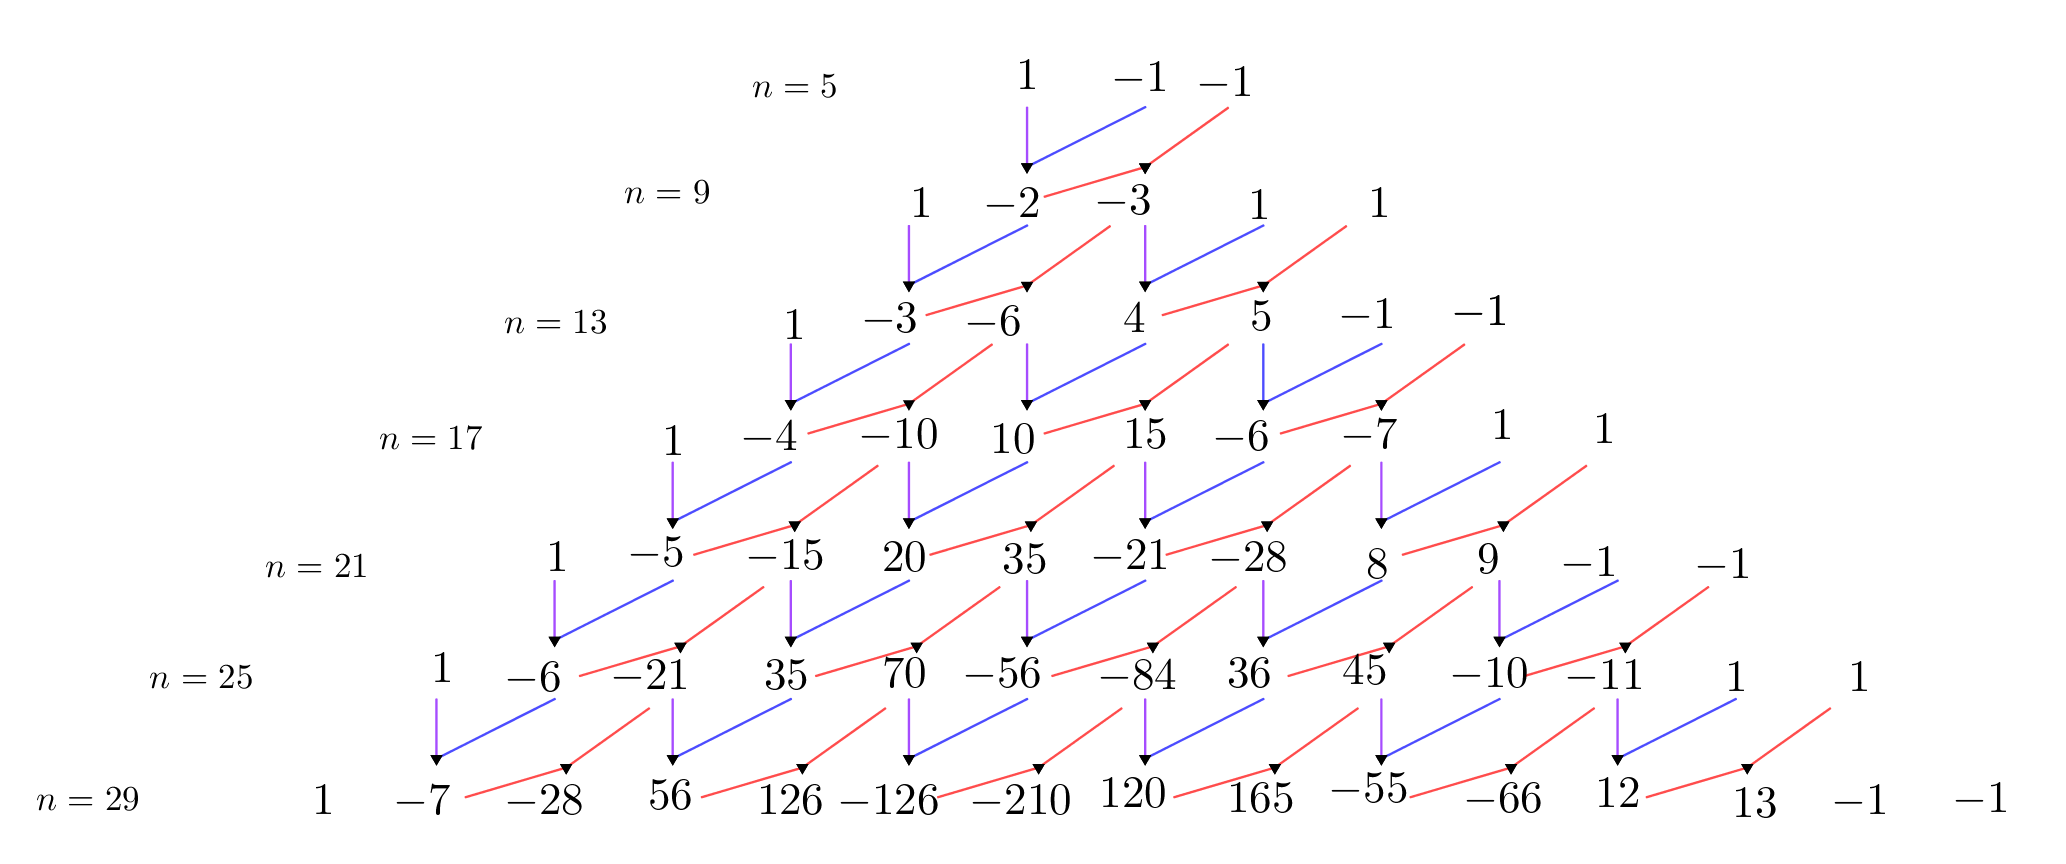
\includegraphics[width=1\textwidth]{ILCFig18_pattern}
			\caption{An array of numbers describing the coefficients of  $q_n (x)$ in standard form.}
\label{fig:pattern}
\end{figure}

\begin{conj}
\label{thm:Conjecture2}
In addition to the previous observation and conjecture, we notice that the roots of the characteristic $p_n (x)$ of $M_n$, at least for the values of $n$ shown in Figure~\ref{fig:pattern}, are given by $\mu_n=\dfrac{1}{s_{n,(n-1)/2}}, -\dfrac{1}{s_{n,(n-3)/2}}, \ldots, \dfrac{1}{s_{n,2}}, -\dfrac{1}{s_{n,1}}, \dfrac{1}{s_{n,0}}=1$. This indicates that each eigenvalue of $M_n$ takes the form $\pm \dfrac{1}{s_{n,j}}$. We conjecture that this holds for all odd $n\geq5$. If this conjecture is correct, then $\mu_n$ is non-Pisot if  $g_n (x)$ is irreducible for odd $n\geq11$, since $\dfrac{1}{s_{n,(n-3)/2}}= \dfrac{1}{2\sin(3\pi/2n)}>1$. 
\end{conj}
